\section{算法视角：缓慢对齐}
\label{sec:algorithm}

第~\ref{sec:data} 节从数据侧分析了 one-shot 增益：查询对学习者的价值由其展开所达到的状态决定。转向算法侧，本节探讨 \textit{为何一次查询能在如此多步中持续产生增益}。

\begin{tcolorbox}[takeawaysbox]
\begin{itemize}[topsep=0pt, partopsep=0pt, leftmargin=12pt, itemsep=0pt]
    \item  \textbf{对齐随时间推移而减缓，且这一趋势与查询次数无关。} 学生模型在整个运行过程中持续缩小教师模型与学生模型之间的差距，但进展速度稳步下降，因此一次运行需要数百步而非数十步。增加查询次数并不会加快或减慢这一过程。

    \item  \textbf{即使是一组固定的状态也需要数百步才能学习完成。}
    一次从头到尾在相同状态上训练的运行仍然需要数百步才能取得改进，因此维持长时间运行并不需要持续提供新的状态。
\end{itemize}
\end{tcolorbox}

\subsection{对齐度量}
\label{sec:rate-setup}

OPD使学生与教师保持一致。在任何时刻，有两个量描述这种一致性的状态：师生之间还剩多少分歧，以及分歧减少的速度。我们通过学生实际访问的状态来衡量这两个量。

\begin{itemize}[topsep=2pt, partopsep=0pt, leftmargin=13pt, itemsep=2pt, parsep=0pt]
    \item  \textbf{距离。} 教师和学生在每个访问位置上意见相左，这种分歧由公式~\ref{eq:token-advantage} 的每个 token 优势决定。我们定义 \emph{距离} \(d_t\) 为学生在步骤 \(t\) 访问的位置 \(\mathcal{T}_t\) 上，该分歧的平均大小：
    \begin{equation}
        d_t
        =
        \frac{1}{|\mathcal{T}_t|}
        \sum_{i\in\mathcal{T}_t}
        \left|
            \log\pi_T(y_i\mid s_i)-\log\pi_{\theta_t}(y_i\mid s_i)
        \right|.
        \label{eq:distance}
    \end{equation}
    此处 \(s_i=(x,y_{<i})\)  是在标记位置 \(i\) 的状态，如第~\ref{sec:prelim}~节所定义。对幅度取平均可防止正负的每个标记间隔相互抵消，因此只有当两个策略在学生访问的位置上达成一致时，\(d_t\)  才会降至零。
    \item  \textbf{吸收率。} \emph{吸收率} \(v_t\)  是每次更新所吸收的距离的比例，
    \begin{equation}
        v_t = \frac{d_t-d_{t+1}}{d_t}.
        \label{eq:absorption-rate}
    \end{equation}
\end{itemize}
我们从第 30 步开始追踪这两个指标，此时梯度裁剪不再起作用。由于每次运行都是在它所访问的状态上测量距离，到那时这些运行已分别达到不同的水平。因此，我们以每次运行在第 30 步的值为基准进行报告，我们称之为 \emph{距离剩余} \(d_t/d_{30}\) 。\footnote{训练后期，连续两个步骤构成的一对数据过于嘈杂，难以读取，因此 \(v_t\)  是在几何窗口 \([t/1.4,\,1.4t]\) 上进行估计的，这就是为何它在步骤 \(300\) 之前停止的原因。附录~\ref{app:alignment-dynamics} 提供了这两种约定背后的估计量和证据。}

\subsection{对齐在各类数据中同样变慢}
\label{sec:mech-dynamics}

我们跟踪在 1、4、16 和全部 DAPO-Math-17k 查询上训练的 OPD 的 \(d_t\) 和 \(v_t\)，经过相同的 \(300\) 步数，并在第~\ref{sec:setup} 节的数学配置下进行。

\begin{figure}[t]
    \centering
    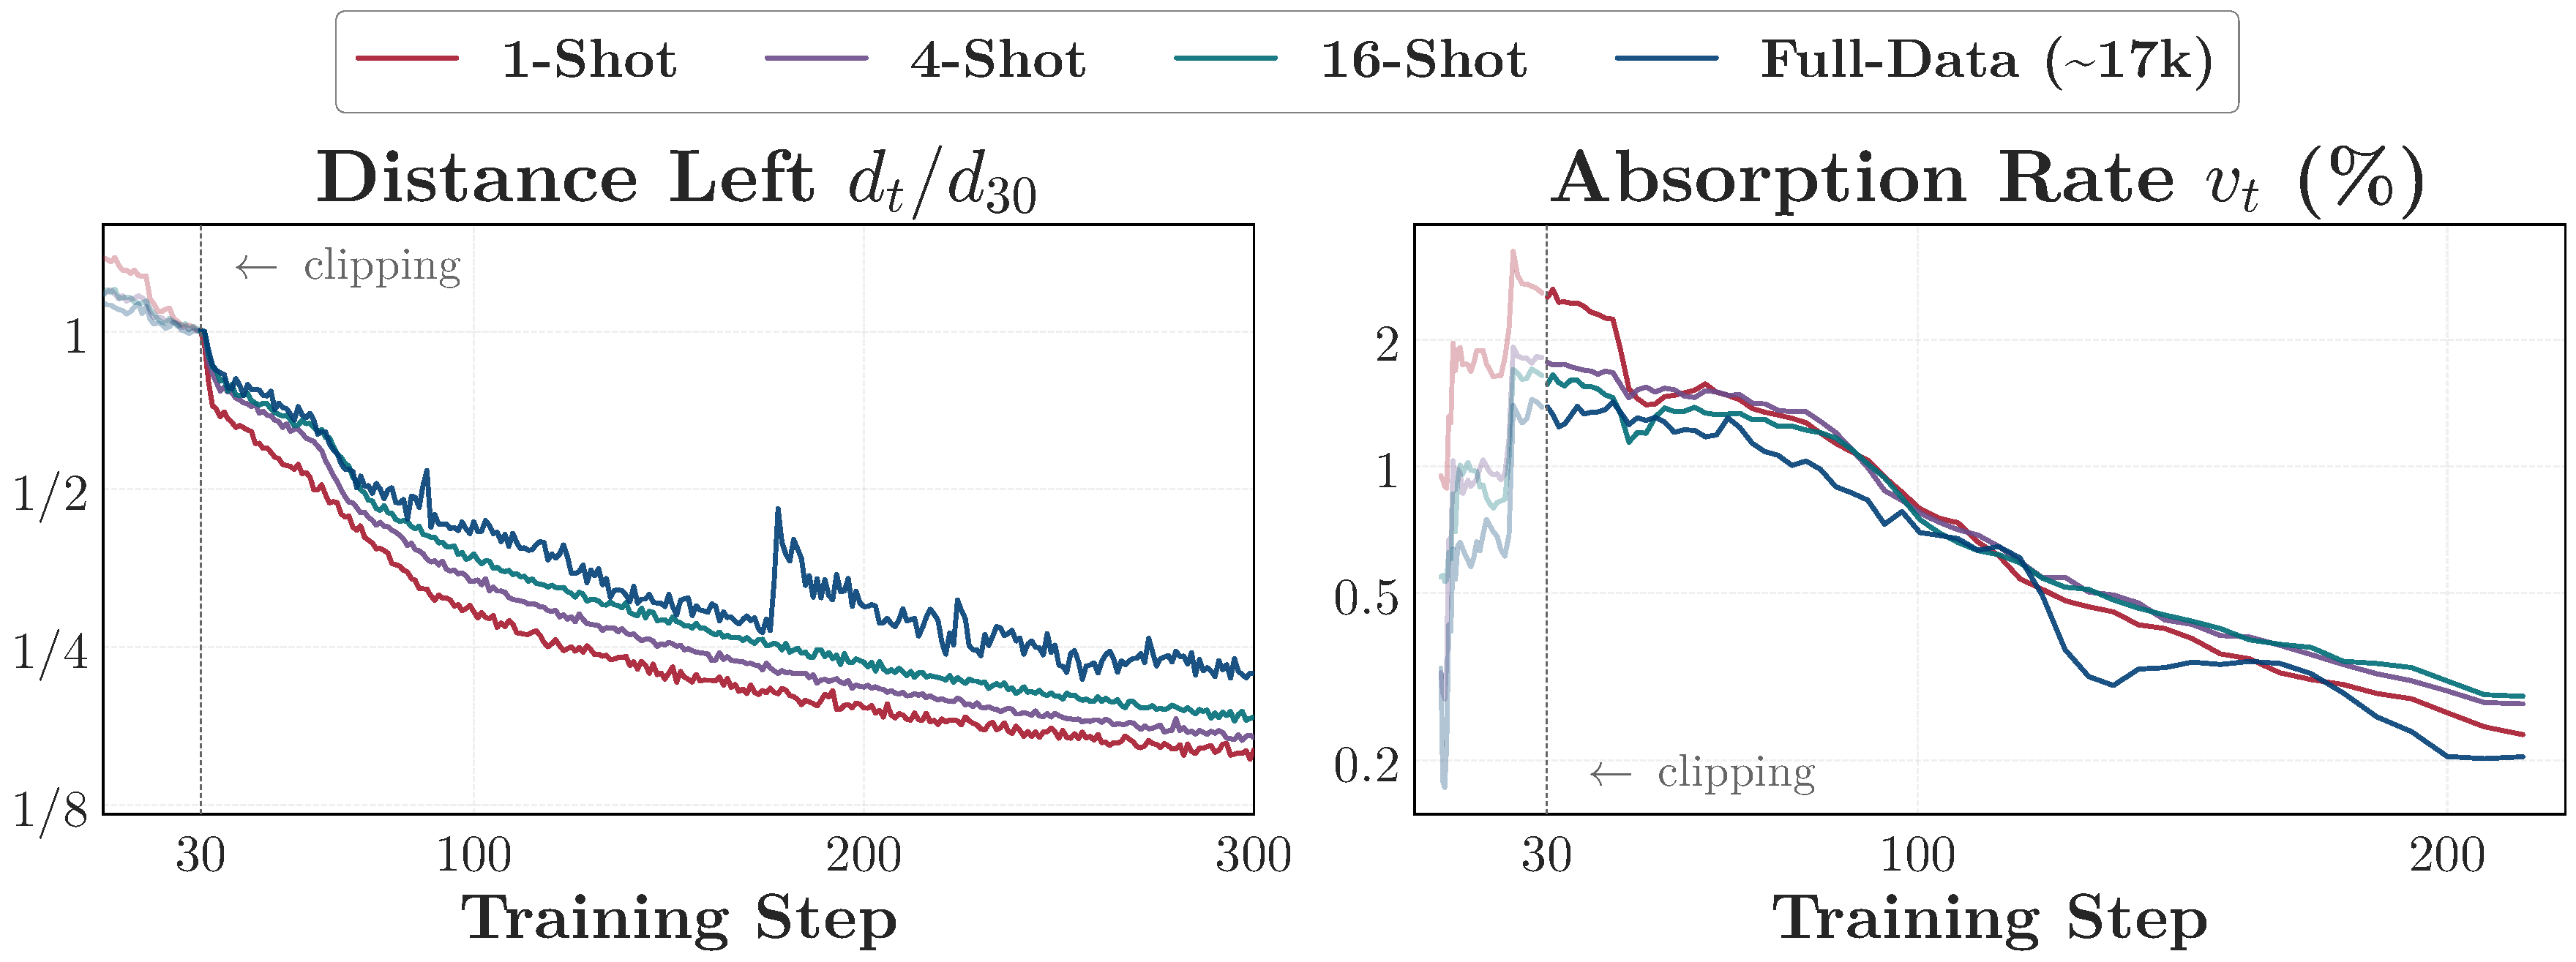
\includegraphics[width=0.75\linewidth]{figures/5_digestion_rate_v2.pdf}
    \caption{
    教师-学生对齐效果，针对在1、4、16及全部DAPO-Math-17k查询上训练的OPD。距离（左）和吸收率（右）均以对数刻度的纵轴相对于线性步长进行展示。
    }
    \label{fig:alignment-contraction}
\end{figure}

\paragraph{学生调整得越来越慢。}
距离在整个过程中持续下降，因此学生从未陷入停滞。减缓的是吸收速率，这在图~\ref{fig:alignment-contraction} 右侧面板中贯穿整个过程不断下降：在左侧的对数距离坐标轴上，恒定速率会呈现为一条直线，而所有四条曲线都变得更为平缓。因此每次更新所吸收的剩余量都比上次少，这就是为什么一次运行需要数百步而非数十步的原因。

\paragraph{吸收率在每个训练集大小下的下降方式大致相同。}
四次运行均以相同方式执行：每次在第 \(78\%\) 步到第 \(84\%\) 步之间，将第 \(30\) 步的距离减少 \(300\) 量，且四次运行在训练过程中均以相似的因子减慢（附录~\ref{app:alignment-dynamics} 提供了各次运行的具体数值以及这些读数所依据的约定）。因此，一次查询不会使对齐过程变慢或变快：速度是 OPD 的属性，而非训练集的属性。学习率仅影响所需步数的多少，而不影响距离下降的方式（附录~\ref{app:lr-sensitivity}）。

\subsection{固定状态下的消融分析}
\label{sec:fixed-states}
同策略训练会随着学生的变化不断产生新的状态，而对数百步的阅读表明，运行时间取决于这一状态供应的持续时间。将训练状态固定下来可以直接检验这一观点：如果一组固定的状态很快被耗尽，那么异策略运行就应该提前结束。

\paragraph{设置}
我们比较了两种仅在训练状态来源上不同的 one-shot 运行。始终同策略运行在每一步都从当前学生处获取新的轨迹。始终异策略运行则重复使用第~\ref{sec:state-diversity}~节中的 \(64\) 轨迹，这些轨迹仅从初始学生采样一次，用于每次更新，因此其训练状态保持固定，而学生则不断变化。

\paragraph{保持状态不变，运行时间仍然相同。}

\begin{figure}[t]
    \centering
    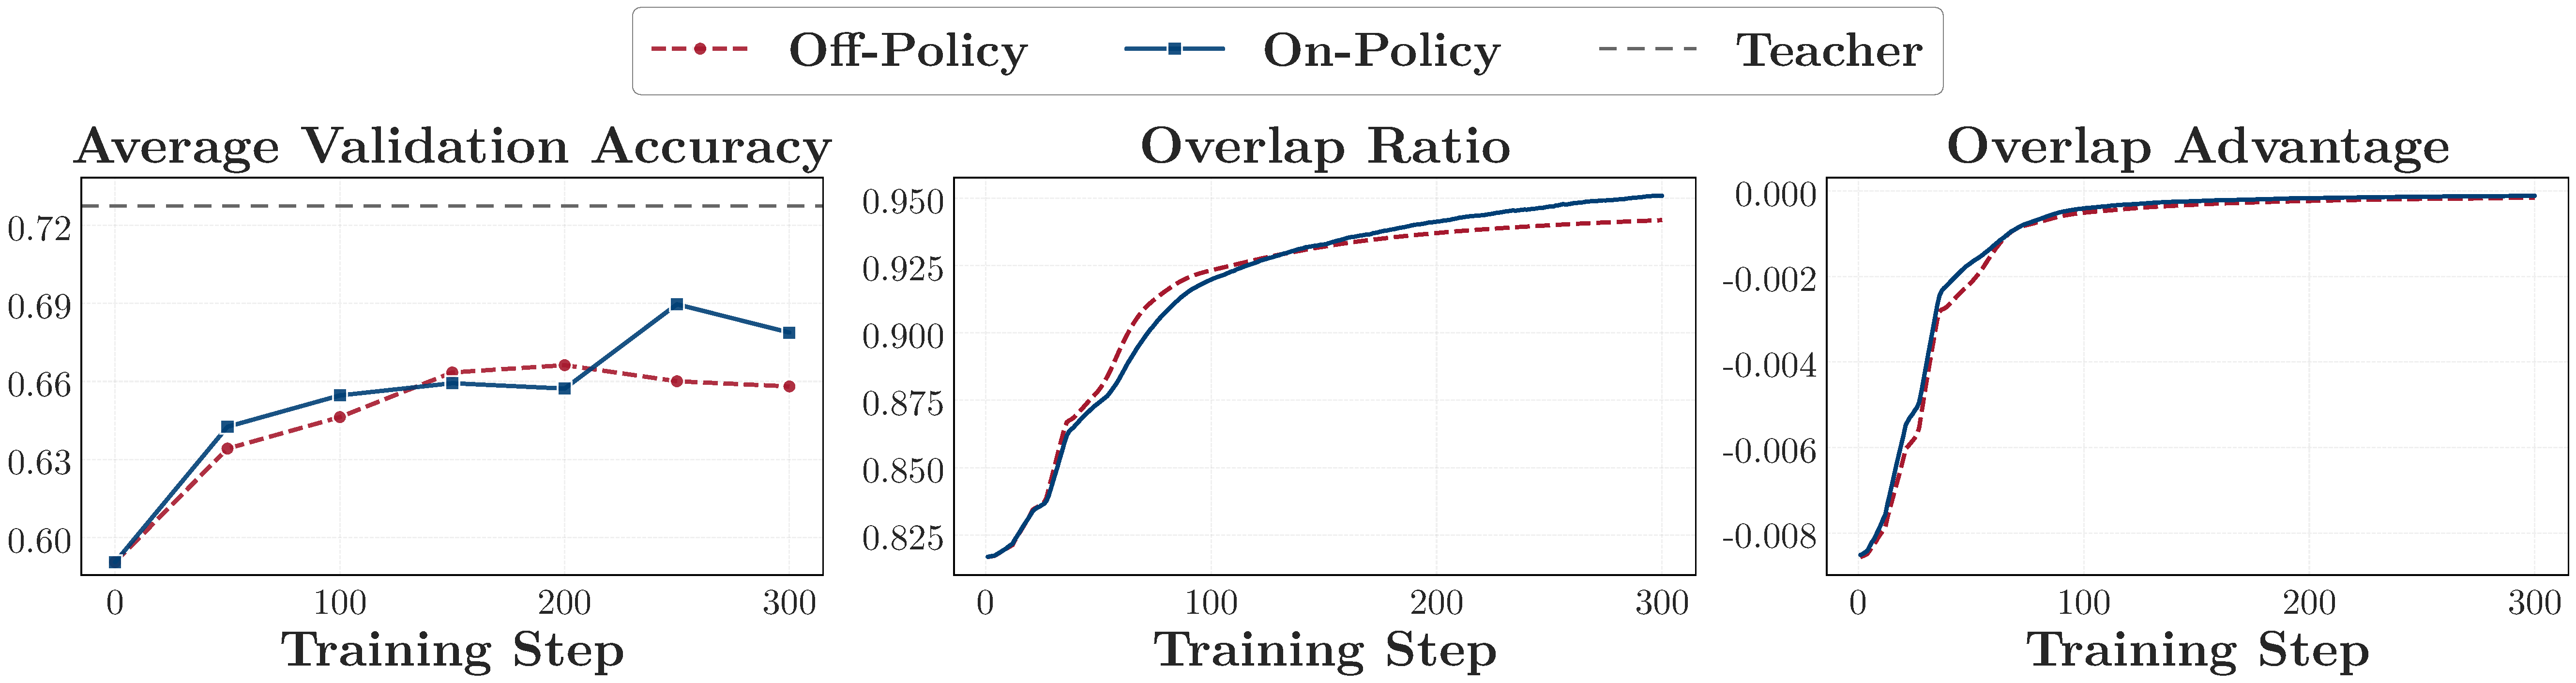
\includegraphics[width=\linewidth]{figures/5_online_offline.pdf}
    \caption{
    同策略和异策略 one-shot 运行的有效准确率和对齐度量。
    }
    \label{fig:online-offline}
\end{figure}
图~\ref{fig:online-offline} 显示，异策略运行的准确率在约 \(200\) 步内稳步提升，随后趋于停滞，因此其增益是在数百步内逐步累积的，而非仅在最初的几次更新中产生。对齐指标的变化同样缓慢：异策略运行的 top-\(16\) token 重叠率上升，且其重叠-token 优势趋近于零，均需经历数百步。因此，移除该状态供给并不会缩短运行长度。  
这表明，一组固定的状态本身已足以维持一次异策略动态（OPD）运行达数百步之久，故运行长度并非由新鲜状态持续到达的时间长短所决定。

